\documentclass{beamer}
\usepackage{amsmath}
\usepackage{physics}
\usepackage{tikz}
\usetikzlibrary{3d,calc}

\title{Ejercicio: El P�ndulo Esf�rico con Barra R�gida}
\author{Curso de Mec�nica Cl�sica}
\date{}

\begin{document}

\frame{\titlepage}

\begin{frame}{Descripci�n del sistema}
\begin{itemize}
  \item Consideramos una barra r�gida de masa \( M \) y longitud \( \ell \), fijada por un extremo.
  \item El centro de masa est� a una distancia \( \ell/2 \) del punto de suspensi�n.
  \item Movimiento libre bajo gravedad en un hemisferio: p�ndulo esf�rico r�gido.
\end{itemize}

\begin{center}
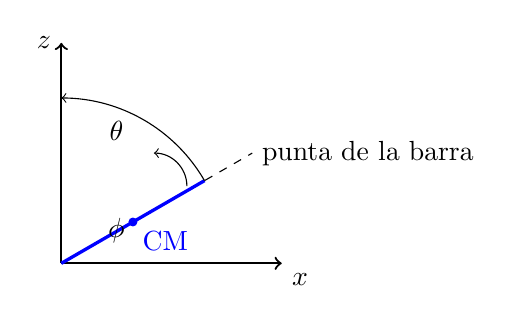
\begin{tikzpicture}[scale=1.4]
  \coordinate (O) at (0,0); % suspension point
  \draw[->, thick] (O) -- (2,0) node[below right] {$x$};
  \draw[->, thick] (O) -- (0,2) node[left] {$z$};
  \draw[dashed] (O) -- (30:2) coordinate (end) node[right] {punta de la barra};

  \draw[very thick, blue] (O) -- (30:1.5);
  \filldraw[blue] (30:0.75) circle (1pt) node[below right] {CM};

  \draw[->] (30:1.5) arc (30:90:1.5);
  \node at (0.5,1.2) {$\theta$};

  \draw[->] (30:1.2) ++(0.1,0.1) arc (0:90:0.3);
  \node at (0.5,0.3) {$\phi$};
\end{tikzpicture}
\end{center}
\end{frame}

\begin{frame}{Parte A: Lagrangiano y coordenadas c�clicas}
\textbf{1.} Determine el Lagrangiano del sistema. Para una barra de masa \( M \), el momento de inercia respecto al punto de suspensi�n es:
\[
I = \frac{1}{3} M \ell^2
\]

\textbf{2.} Escriba:
\[
L = \frac{1}{2} I (\dot{\theta}^2 + \sin^2 \theta \dot{\phi}^2) + Mg \frac{\ell}{2} \cos \theta
\]

\textbf{3.} �Cu�l es la coordenada c�clica? �Qu� cantidad se conserva?
\end{frame}

\begin{frame}{Parte B: Primeras integrales}
\textbf{4.} Usando la conservaci�n de la energ�a, escriba la ecuaci�n del movimiento:
\[
\frac{1}{2} I \dot{\theta}^2 + V_{\text{ef}}(\theta) = E
\]
\[
V_{\text{ef}}(\theta) = \frac{p_\phi^2}{2 I \sin^2 \theta} - Mg \frac{\ell}{2} \cos \theta
\]

\textbf{5.} Discuta el papel del momento angular \( p_\phi \) en el confinamiento del movimiento.
\end{frame}

\begin{frame}{Parte C: Movimiento en un plano}
\begin{itemize}
  \item �Qu� condici�n sobre \( p_\phi \) garantiza que la barra oscile en un solo plano?
  \item Interprete f�sicamente \( \phi = \text{cte} \): �cu�l es el plano del movimiento?
  \item �Qu� rol juega la simetr�a azimutal rota?
\end{itemize}
\end{frame}

\begin{frame}{Objetivos del ejercicio}
\begin{itemize}
  \item Aplicar coordenadas generalizadas a un cuerpo r�gido con simetr�a axial.
  \item Distinguir entre coordenadas c�clicas y no c�clicas.
  \item Interpretar el potencial efectivo en un sistema rotacional.
  \item Contrastar este sistema con el trompo sim�trico de Lagrange.
\end{itemize}
\end{frame}

\end{document}
